\documentclass[11pt,a4paper]{article}
\usepackage[margin=2.5cm]{geometry}
\usepackage{booktabs}
\usepackage{listings}
\usepackage{xcolor}
\usepackage{graphicx}
\usepackage{float}

\lstset{
  basicstyle=\ttfamily\small,
  frame=single,
  backgroundcolor=\color{gray!8},
  breaklines=true
}

\title{Labwork 3: Hello, CUDA!}
\author{Yanis Denizot -- 2640051}
\date{\today}

\begin{document}
\maketitle

\section{Objective}
The goal of this labwork is to convert a color RGB image to grayscale, first on the CPU
with a simple loop, then on the GPU with Numba CUDA, and to compare the time of both
versions. I also tested different block sizes to see how they change the GPU time.

\section{Environment}
I ran the code on Google Colab with an NVIDIA Tesla T4 GPU (40 SM, compute capability 7.5).
The input image is a color JPEG of $471 \times 651$ pixels, so $306\,621$ pixels in total.

\section{Implementation}

\subsection{Loading the image}
I load the image with \texttt{matplotlib.pyplot.imread}. It gives an array of shape
$(651, 471, 3)$ with type \texttt{uint8} (values from 0 to 255). Then I flatten it with
\texttt{reshape(pixelCount, 3)} to get a 1D list of pixels, where each pixel has its R, G
and B values. This way each pixel has a unique index, which is easier to use on the GPU.

For the grayscale value, I use the simplest formula, the average of the 3 channels:
\[
g = \frac{R + G + B}{3}
\]

\subsection{CPU version}
On the CPU, I use a \texttt{for} loop over all the pixels, one by one. I convert the values
to \texttt{int} before the sum, because with \texttt{uint8} the sum can go above 255 and
overflow, which gives wrong colors.

\begin{lstlisting}[language=Python]
grayCPU = np.zeros((pixelCount, 3), np.uint8)
for i in range(pixelCount):
    g = (int(flat[i, 0]) + int(flat[i, 1]) + int(flat[i, 2])) // 3
    grayCPU[i, 0] = g
    grayCPU[i, 1] = g
    grayCPU[i, 2] = g
\end{lstlisting}

\subsection{GPU version}
On the GPU, there is no loop: the kernel is executed by many threads at the same time, and
each thread processes one pixel. Each thread computes its pixel index from its position in
the block and the index of its block:
\[
\texttt{tidx} = \texttt{threadIdx.x} + \texttt{blockIdx.x} \times \texttt{blockDim.x}
\]

\begin{lstlisting}[language=Python]
@cuda.jit
def grayscale(src, dst):
    tidx = cuda.threadIdx.x + cuda.blockIdx.x * cuda.blockDim.x
    if tidx < src.shape[0]:
        g = np.uint8((src[tidx, 0] + src[tidx, 1] + src[tidx, 2]) / 3)
        dst[tidx, 0] = g
        dst[tidx, 1] = g
        dst[tidx, 2] = g
\end{lstlisting}

The steps are:
\begin{enumerate}
  \item Copy the image to the GPU memory with \texttt{cuda.to\_device}, and allocate the
        output with \texttt{cuda.device\_array}.
  \item Launch the kernel with \texttt{grayscale[gridSize, blockSize](devSrc, devDst)}.
  \item Copy the result back to the CPU with \texttt{copy\_to\_host}.
\end{enumerate}

The number of blocks is rounded up, so that all the pixels are covered:
\begin{lstlisting}[language=Python]
gridSize = (pixelCount + blockSize - 1) // blockSize
\end{lstlisting}
Because of this, the last block can have more threads than remaining pixels. This is why
the kernel checks \texttt{if tidx < src.shape[0]}, so the extra threads do nothing instead
of reading outside the array.

\subsection{Time measurement}
I use \texttt{time.time()}. Two details are important for the GPU:
\begin{itemize}
  \item The first launch of a kernel is slow because Numba compiles it. So I launch the
        kernel once before measuring (warm-up).
  \item A kernel launch is asynchronous: Python does not wait for the GPU to finish. So I
        call \texttt{cuda.synchronize()} before stopping the timer.
\end{itemize}
The GPU time only measures the kernel, not the copies between CPU and GPU memory.

\section{Results}

\subsection{Grayscale images}
The CPU and GPU results are exactly the same (the two output files are identical).

\begin{figure}[H]
\centering
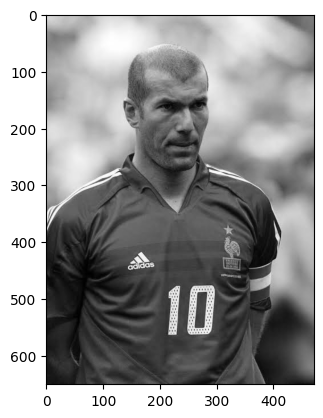
\includegraphics[width=0.45\textwidth]{gray_cpu.png}
\hfill
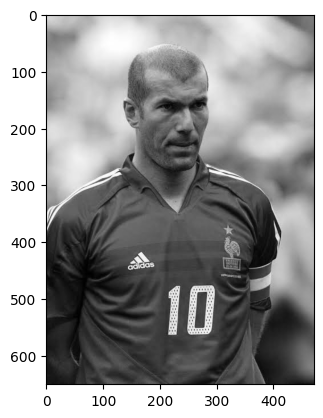
\includegraphics[width=0.45\textwidth]{gray_gpu.png}
\caption{Grayscale result on CPU (left) and on GPU (right)}
\end{figure}

\subsection{Speedup}

\begin{table}[H]
\centering
\begin{tabular}{lr}
\toprule
\textbf{Version} & \textbf{Time} \\
\midrule
CPU (for loop)             & 0.3957 s \\
GPU (block size 64)        & 0.000404 s \\
\midrule
\textbf{Speedup}           & \textbf{$\approx$ 979} \\
\bottomrule
\end{tabular}
\caption{CPU vs GPU time for $306\,621$ pixels}
\end{table}

The GPU is about 979 times faster than the CPU. This GPU time comes from only one launch,
so it is not very precise. With the average over 100 launches (next section), the kernel
takes about 0.078 ms, so the real speedup of the kernel is even higher (around 5000).

\subsection{Block size vs time}
For each block size, I launched the kernel 100 times and took the average time.

\begin{table}[H]
\centering
\begin{tabular}{rr}
\toprule
\textbf{Block size} & \textbf{Time ($\mu$s)} \\
\midrule
32   & 91.4 \\
64   & 78.4 \\
128  & 77.9 \\
256  & 78.1 \\
512  & 78.3 \\
1024 & 88.3 \\
\bottomrule
\end{tabular}
\caption{Average kernel time for each block size}
\end{table}

\begin{figure}[H]
\centering
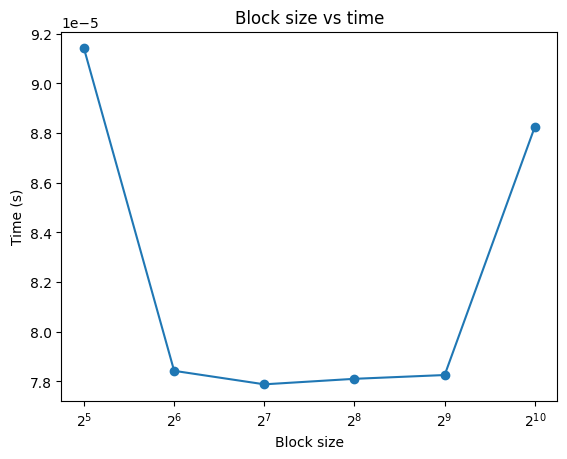
\includegraphics[width=0.7\textwidth]{blocksize_vs_time.png}
\caption{Block size vs time (the x axis is in log scale)}
\end{figure}

\section{Discussion}
The graph has a ``U'' shape: small and very large blocks are slower, and the block sizes
in the middle are the fastest.

\begin{itemize}
  \item \textbf{Block size 32 is slow.} On the T4 (compute capability 7.5), one SM can run
        at most 16 blocks and 1024 threads at the same time. With blocks of 32 threads, an
        SM can only have $16 \times 32 = 512$ threads, so half of the SM is not used.
  \item \textbf{Block sizes 64 to 512 are the fastest.} With these sizes the SM can be
        full: for example $16 \times 64 = 1024$ or $8 \times 128 = 1024$ threads.
        The times are almost the same, and the best one is 128.
  \item \textbf{Block size 1024 is slower.} One block takes the whole SM, so the SM has to
        wait for all the 1024 threads of the block to finish before it can start a new
        block. With smaller blocks, a new block can start as soon as one block finishes.
\end{itemize}

The difference between the best and the worst block size is about 15\%. It looks bigger on
the graph because the y axis does not start at zero. In a first test with only 10 launches,
the results were noisy (block size 64 looked like the slowest), because the kernel time is
very small (less than 0.1 ms). Using the average over 100 launches gave stable results.

\section{Conclusion}
The GPU version gives the same image as the CPU version, but it is much faster (about 979
times on one launch), because thousands of threads process the pixels at the same time.
For this kernel on the Tesla T4, a block size between 64 and 512 gives the best time.

\end{document}
